\chapter{Background}\label{chapter:background}

Before diving into the details of the main objective of the thesis, it is important to understand some background knowledge. In this chapter i will introduce some necessary detailed background of the rise of \ac{ML}, and how the concenpt of \ac{MLOps} came to be.

\section{The Rise of Machine Learning}
\subsection{The Birth of Machine Learning (1950s)}
The foundations of machine learning were laid in the 1950s by computer scientists and mathematicians who sought to develop algorithms that could enable computers to learn from data \cite{MLHistory, Rahal2024, MLRise}. During this era, several key milestones shaped the field. Such as the Perceptron Algorithm - one of the earliest breakthroughs in machine learning - by Frank Rosenblatt \cite{Frank_Rosenblatt},  was an early form of an artificial neural network, it became the building block for future advancements.
Where he formulated a serie of machines, each serves to interduce a new concept. It aimed to mimic the way biological neurons process information.

\subsection{Resurgence and New Techniques (1980s-1990s)}
An \ac{AI} winter started in the 1970s, that was described as a chain reaction much the same as a nuclear winter, that began with pessimisum in the \ac{AI} community, followed by cutback in fundings, which in turn resulted in end of serious research. After the \ac{AI} winter, machine learning was resurrected in the 1980s and 1990s. New techniques brought to the light, such as
\ac{NN} where Researchers were inspired by the human brain’s structure, according to Geoffrey Hinton \cite{Geoffrey_Hinton}
% TODO add a quote for Geoffrey Hinton
% "I get very excited when we discover a way of making neural networks better - and when that's closely related to how the brain works."
, often referred to as the “father of Deep Learning,”, who made significant contributions during this time.

\subsection{The Rise of Big Data (2000s)}
The 2000s witnessed the rise of big data and the availability of vast amounts of data for training machine learning models.
This era witnessed the emergance of new techniques to be able to deal with vast amount of data, such as,
Data-Driven Approaches \cite{Data-Driven-Approach, Data-Driven-Approach-2}, where machine learning algorithms learned patterns directly from large datasets, and Supervised Learning Dominance, where models learn from labeled examples.
Techniques like regression and classification gained prominence.

\subsection{Deep Learning and Beyond (2010s)}
The 2010s marked a transformative period for machine learning, where the term Deep learning was first introduced
, it it was defined as a subfield of machine learning. other powerful methods were perfected in this era such as \ac{CNN} for image recognition and recurrent neural networks for sequential data revolutionized various domains.

\subsection{State-of-the-Art Machine Learning (Present and Future)}
Nowadays machine learning has made far-reaching changes in various applications across industries.
Machine learning is applied in healthcare, fraud detection, speech recognition, autonomous vehicles, recommendation systems, and more (\autoref{fig:machine_learning_applications} shows some applications of machine learning).
It revolutionizes industries and improves efficiency. However, researchers continue to push boundaries, aiming for \ac{AI} systems that understand context, and are looking forward for the exciting possibilities ahead.
\begin{figure}[htbp]
    \centering
    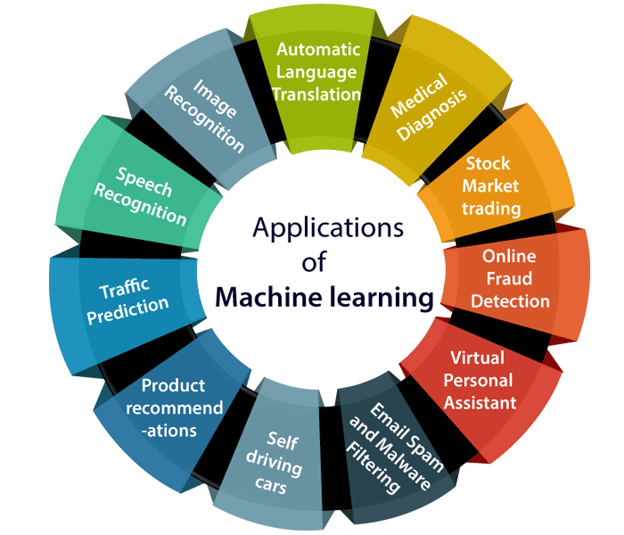
\includegraphics[width=0.5\linewidth]{figures/machine-learning-applications.png}
    \caption{Few applications of machine learning.}
    \label{fig:machine_learning_applications}
\end{figure}

%% here was reached
% TODO rewrite this part
% https://www.ibm.com/blog/mlops-and-the-evolution-of-data-science/
\section{The Evolution of MLOps}
With the rise of machine learning, so did the need for efficient operations around it. This led to the evolution of \ac{MLOps}
\ac{MLOps} is an engineering practice that aims at making the process of deploying machine learning models more efficient, reliable, and maintainable.
It uses \ac{CI/CD} and machine learning models to rationalize the monitoring, deployment and maintenance of machine learning systems.

\subsection{Key Components of MLOps}

As the datasets to train machine learning models got bigger and more complex, the realization for the need of \ac{ML} life cycle grow, as the old techniques weere slow and difficult to scale.
Data scientists worked together with IT teams to create and develop an assembly line for each step of training machine learning models.
In this chapter I will discuss few steps of michine learning life cycle that are crucial for \ac{MLOps} process.
\begin{itemize}
\item \textbf{Data Collection}: Gathering and refining relevant data set from different sources to prepare it for modeling is one of the key components of ML life cycle.
\item \textbf{Building and training}: This is the step  where models are created and trained using data, that were prepared in the previous step. It involves selecting appropriate algorithms and preprocessing the data.
\end{itemize}
And more as shown in \autoref{fig:machine_learning_lifecycle}.
\begin{figure}[htbp]
    \centering
    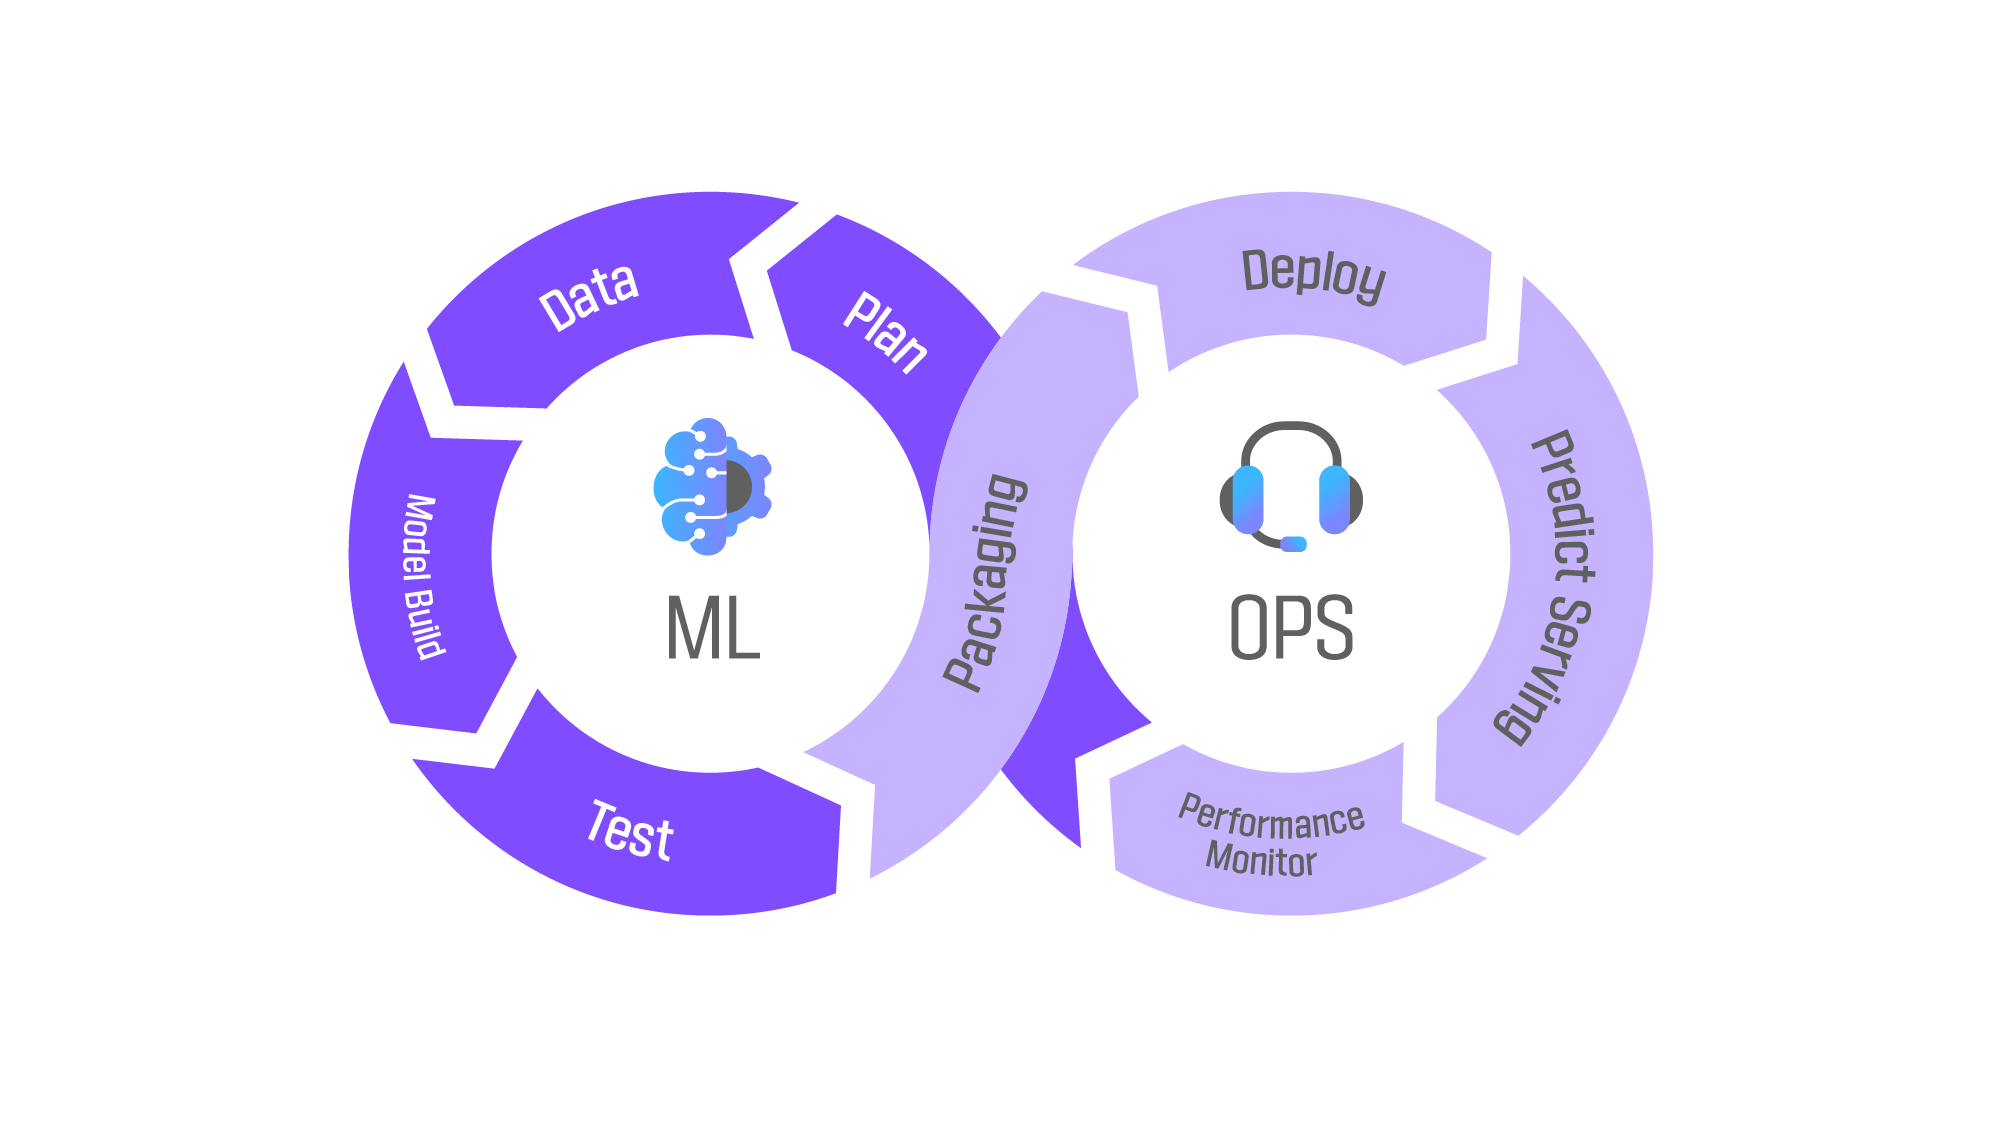
\includegraphics[width=0.78\linewidth]{figures/machine-learning-life-cycle.png}
    \caption{machine learning life cycle.}
    \label{fig:machine_learning_lifecycle}
\end{figure}

\subsection{Comparing MLOps and DevOps}

DevOps is a method which aims at bringing together software development and operations, it shortens the system's development life cycle and provides a continu delivery to a high software quality. 
\newline
\ac{MLOps} does, however, borrow from the DevOps principles of a rapid, continuous approach to writing and updating applications, in that they both have a code-validate-deploy loop. But the \ac{MLOps} life cycle contains additional steps, that are necessary for building and training the machine learning model as shown in \autoref{fig:DevOps_To_MLOPs}.
The aim in both cases is to take the project to production more efficiently with faster fixes, faster releases and ultimately, a higher quality product that boosts customer satisfaction, whether that’s software or machine learning models.
\begin{figure}[htbp]
    \centering
    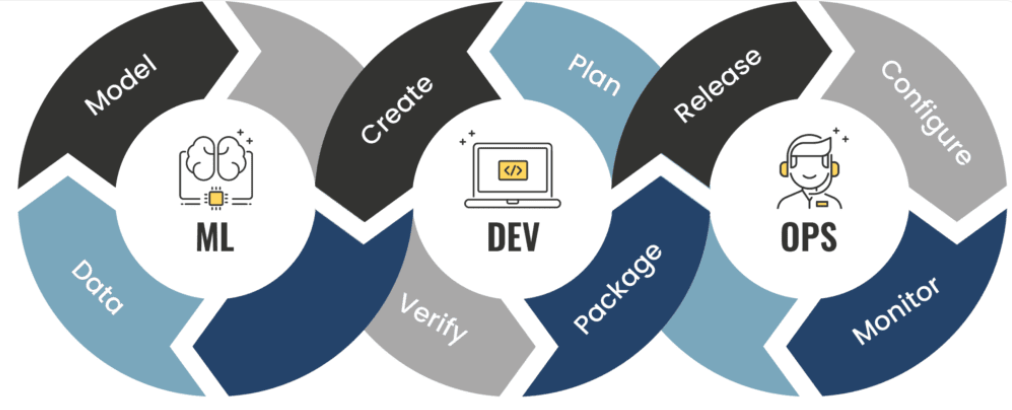
\includegraphics[width=0.78\linewidth]{figures/DevOps-To_MLOps.png}
    \caption{The transition from DevOps to MLOps life cycle.}
    \label{fig:DevOps_To_MLOPs}
\end{figure}
\newline
In this thesis, I delve into these aspects, aiming to bridge the gap between local ML implementation and successful code execution in production systems. Let us embark on this journey toward efficient \ac{MLOps} practices.